\chapter{Algoritmos de árboles}

\index{árbol}

Un \key{árbol} es un grafo conectado y acíclico
que consta de $n$ nodos y $n-1$ aristas.
Eliminar cualquier arista de un árbol lo divide
en dos componentes,
y agregar cualquier arista a un árbol crea un ciclo.
Además, siempre hay un camino único entre cualquieras
dos nodos de un árbol.

Por ejemplo, el siguiente árbol consta de 8 nodos y 7 aristas:
\begin{center}
    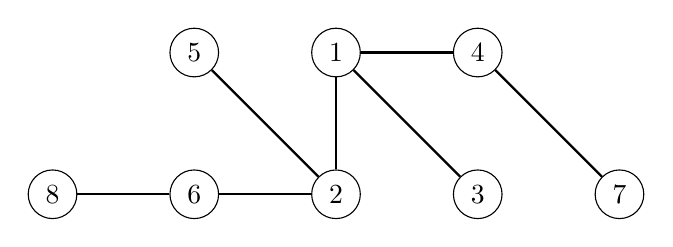
\begin{tikzpicture}[scale=0.9]
        \node[draw, circle] (1) at (0,3) {$1$};
        \node[draw, circle] (2) at (2,3) {$4$};
        \node[draw, circle] (3) at (0,1) {$2$};
        \node[draw, circle] (4) at (2,1) {$3$};
        \node[draw, circle] (5) at (4,1) {$7$};
        \node[draw, circle] (6) at (-2,3) {$5$};
        \node[draw, circle] (7) at (-2,1) {$6$};
        \node[draw, circle] (8) at (-4,1) {$8$};
        \path[draw,thick,-] (1) -- (2);
        \path[draw,thick,-] (1) -- (3);
        \path[draw,thick,-] (1) -- (4);
        \path[draw,thick,-] (2) -- (5);
        \path[draw,thick,-] (3) -- (6);
        \path[draw,thick,-] (3) -- (7);
        \path[draw,thick,-] (7) -- (8);
    \end{tikzpicture}
\end{center}

\index{hoja}

Las \key{hojas} de un árbol son los nodos
con grado 1, es decir, con un único vecino.
Por ejemplo, las hojas del árbol anterior
son los nodos 3, 5, 7 y 8.

\index{raíz}
\index{árbol con raíz}

En un \key{árbol con raíz}, uno de los nodos
se designa como la \key{raíz} del árbol,
y todos los demás nodos son
colocados debajo de la raíz.
Por ejemplo, en el siguiente árbol,
el nodo 1 es el nodo raíz.

\begin{center}
    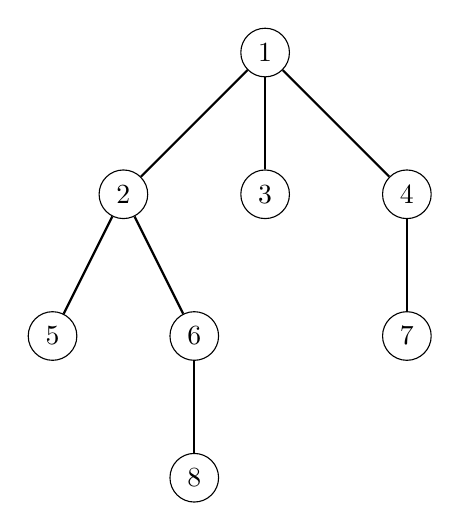
\begin{tikzpicture}[scale=0.9]
        \node[draw, circle] (1) at (0,3) {$1$};
        \node[draw, circle] (4) at (2,1) {$4$};
        \node[draw, circle] (2) at (-2,1) {$2$};
        \node[draw, circle] (3) at (0,1) {$3$};
        \node[draw, circle] (7) at (2,-1) {$7$};
        \node[draw, circle] (5) at (-3,-1) {$5$};
        \node[draw, circle] (6) at (-1,-1) {$6$};
        \node[draw, circle] (8) at (-1,-3) {$8$};
        \path[draw,thick,-] (1) -- (2);
        \path[draw,thick,-] (1) -- (3);
        \path[draw,thick,-] (1) -- (4);
        \path[draw,thick,-] (2) -- (5);
        \path[draw,thick,-] (2) -- (6);
        \path[draw,thick,-] (4) -- (7);
        \path[draw,thick,-] (6) -- (8);
    \end{tikzpicture}
\end{center}
\index{hijo}
\index{padre}

En un árbol con raíz, los \key{hijos} de un nodo
son sus vecinos inferiores, y el \key{padre} de un nodo
es su vecino superior.
Cada nodo tiene exactamente un padre,
excepto la raíz, que no tiene padre.
Por ejemplo, en el árbol anterior,
los hijos del nodo 2 son los nodos 5 y 6,
y su padre es el nodo 1.

\index{subárbol}

La estructura de un árbol con raíz es \emph{recursiva}:
cada nodo del árbol actúa como la raíz de un \key{subárbol}
que contiene el propio nodo y todos los nodos
que están en los subárboles de sus hijos.
Por ejemplo, en el árbol anterior, el subárbol del nodo 2
consta de los nodos 2, 5, 6 y 8:
\begin{center}
    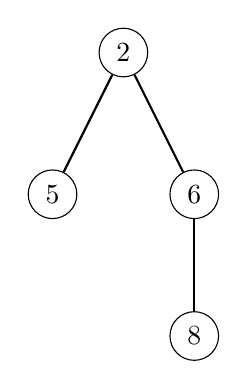
\begin{tikzpicture}[scale=0.9]
        \node[draw, circle] (2) at (-2,1) {$2$};
        \node[draw, circle] (5) at (-3,-1) {$5$};
        \node[draw, circle] (6) at (-1,-1) {$6$};
        \node[draw, circle] (8) at (-1,-3) {$8$};
        \path[draw,thick,-] (2) -- (5);
        \path[draw,thick,-] (2) -- (6);
        \path[draw,thick,-] (6) -- (8);
    \end{tikzpicture}
\end{center}

\section{Recorrido de árboles}

Siempre podemos utilizar algoritmos generales de recorrido de grafos
para recorrer los nodos de un árbol. Sin embargo, el recorrido
de un árbol es más fácil de implementar que aquel de un grafo general,
porque en un árbol no hay ciclos y no es posible alcanzar un nodo
desde múltiples direcciones.

La fórma típica de recorrer un árbol es comenzar una búsqueda en
profundidad en un nodo arbitrario. La siguiente función recursiva
puede ser utilizada:

\begin{lstlisting}
void dfs(int s, int p) {
    // procesar nodo s
    for (auto u : ady[s]) {
        if (u != p) dfs(u, s);
    }
}
\end{lstlisting}

La función recibe dos parámetros: el nodo actual $s$ y el nodo
previo o padre $p$. El propósito del parámetro $p$ es asegurarse de que
la búsqueda solo alcance nodos que todavía no hayan sido visitados.

La siguiente llamada comienza la búsqueda en el nodo $x$:

\begin{lstlisting}
dfs(x, 0);
\end{lstlisting}

En la primera llamada, $p=0$, porque no hay ningún nodo previo,
y está permitido seguir en cualquier dirección dentro del árbol.

\subsubsection{Programación dinámica}

Podemos utilizar la programación dinámica para calcular información
durante el recorrido de un árbol. Usando la programación dinámica
podemos, por ejemplo, calcular en $O(n)$, para cada nodo de un árbol
con raíz, el número de nodos en su subárbol, o la longitud del
camino más largo desde el nodo a una hoja.

Como ejemplo, calculemos para cada nodo $s$ el valor $\texttt{conteo}[s]$:
el número de nodos en su subárbol. El subárbol contiene el nodo en sí
y todos los nodos en los subárboles de sus hijos, así que podemos
calcular el número de nodos recursivamente con el siguiente código:

\begin{lstlisting}
void dfs(int s, int p) {
    count[s] = 1;
    for (auto u : adj[s]) {
        if (u == p) continue;
        dfs(u, s);
        count[s] += count[u];
    }
}
\end{lstlisting}

\section{Diámetro de un árbol}

\index{diámetro}

El \key{diámetro} de un árbol es la longitud máxima de un
camino entre dos nodos. Por ejemplo, considera el siguiente árbol:
\begin{center}
    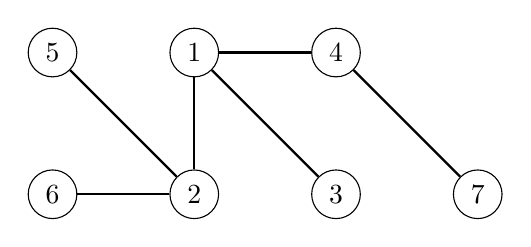
\begin{tikzpicture}[scale=0.9]
        \node[draw, circle] (1) at (0,3) {$1$};
        \node[draw, circle] (2) at (2,3) {$4$};
        \node[draw, circle] (3) at (0,1) {$2$};
        \node[draw, circle] (4) at (2,1) {$3$};
        \node[draw, circle] (5) at (4,1) {$7$};
        \node[draw, circle] (6) at (-2,3) {$5$};
        \node[draw, circle] (7) at (-2,1) {$6$};
        \path[draw,thick,-] (1) -- (2);
        \path[draw,thick,-] (1) -- (3);
        \path[draw,thick,-] (1) -- (4);
        \path[draw,thick,-] (2) -- (5);
        \path[draw,thick,-] (3) -- (6);
        \path[draw,thick,-] (3) -- (7);
    \end{tikzpicture}
\end{center}

El diámetro de este árbol es 4, que corresponde al siguiente camino:
\begin{center}
    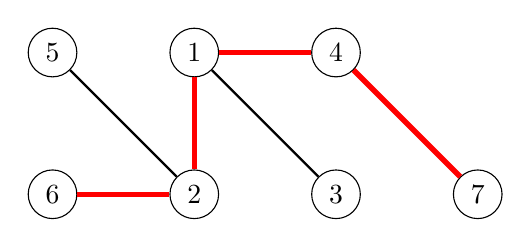
\begin{tikzpicture}[scale=0.9]
        \node[draw, circle] (1) at (0,3) {$1$};
        \node[draw, circle] (2) at (2,3) {$4$};
        \node[draw, circle] (3) at (0,1) {$2$};
        \node[draw, circle] (4) at (2,1) {$3$};
        \node[draw, circle] (5) at (4,1) {$7$};
        \node[draw, circle] (6) at (-2,3) {$5$};
        \node[draw, circle] (7) at (-2,1) {$6$};
        \path[draw,thick,-] (1) -- (2);
        \path[draw,thick,-] (1) -- (3);
        \path[draw,thick,-] (1) -- (4);
        \path[draw,thick,-] (2) -- (5);
        \path[draw,thick,-] (3) -- (6);
        \path[draw,thick,-] (3) -- (7);

        \path[draw,thick,-,color=red,line width=2pt] (7) -- (3);
        \path[draw,thick,-,color=red,line width=2pt] (3) -- (1);
        \path[draw,thick,-,color=red,line width=2pt] (1) -- (2);
        \path[draw,thick,-,color=red,line width=2pt] (2) -- (5);
    \end{tikzpicture}
\end{center}
Ten en cuenta que puede haber múltiples caminos de camino máximo.
En el camino de arriba, podríamos reemplazar el nodo 6 por el nodo 5
para obtener otro camino de longitud 4.

Ahora veremos dos algoritmos de tiempo $O(n)$ para calcular el
diámetro de un árbol. El primer algoritmo se basa en la programación
dinámica, y el segundo algoritmo utiliza dos búsquedas en profundidad.

\subsubsection{Algoritmo 1}

Una manera general de abordar muchos problemas en árboles comienza
con asignarles una raíz arbitrariamente. Luego de esto, podemos
intentar resolver el problema por separado en cada subárbol. Nuestro
primer algoritmo para calcular el diámetro se basa en esta idea.

Una observación importante es que cada camino en un árbol con raíz
tiene un \emph{punto más alto}: el nodo de máxima altura que pertenece
al camino. Por ende podemos calcular, para cada nodo, la longitud
del camino máximo cuyo punto más alto es el nodo. Uno de esos caminos
corresponde al diámetro del árbol.

Por ejemplo, en el siguiente árbol, el nodo 1 es el punto más alto
en el camino que corresponde al diámetro:
\begin{center}
    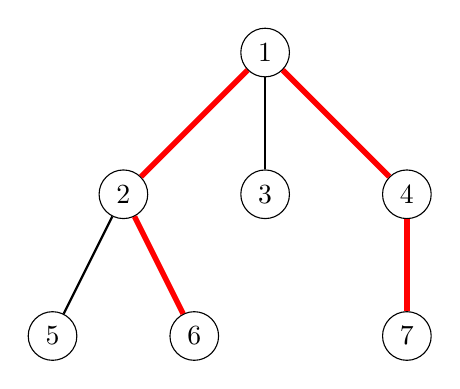
\begin{tikzpicture}[scale=0.9]
        \node[draw, circle] (1) at (0,3) {$1$};
        \node[draw, circle] (2) at (2,1) {$4$};
        \node[draw, circle] (3) at (-2,1) {$2$};
        \node[draw, circle] (4) at (0,1) {$3$};
        \node[draw, circle] (5) at (2,-1) {$7$};
        \node[draw, circle] (6) at (-3,-1) {$5$};
        \node[draw, circle] (7) at (-1,-1) {$6$};
        \path[draw,thick,-] (1) -- (2);
        \path[draw,thick,-] (1) -- (3);
        \path[draw,thick,-] (1) -- (4);
        \path[draw,thick,-] (2) -- (5);
        \path[draw,thick,-] (3) -- (6);
        \path[draw,thick,-] (3) -- (7);

        \path[draw,thick,-,color=red,line width=2pt] (7) -- (3);
        \path[draw,thick,-,color=red,line width=2pt] (3) -- (1);
        \path[draw,thick,-,color=red,line width=2pt] (1) -- (2);
        \path[draw,thick,-,color=red,line width=2pt] (2) -- (5);
    \end{tikzpicture}
\end{center}

Para cada nodo $x$ podemos calcular dos valores:
\begin{itemize}
    \item $\texttt{a\_hoja}(x)$: la longitud máxima de un camino
          desde $x$ a cualquier hoja
    \item $\texttt{long\_max}(x)$: la longitud máxima de un camino
          cuyo punto más alto es $x$
\end{itemize}

Por ejemplo, en el árbol de arriba, $\texttt{a\_hoja}(1)=2$, porque
hay un camino $1 \rightarrow 2 \rightarrow 6$, y $\texttt{long\_max}(1)=4$,
porque hay un camino
$6 \rightarrow 2 \rightarrow 1 \rightarrow 4 \rightarrow 7$.
En este caso, $\texttt{long\_max}(1)$ es igual al diámetro.

La programación dinámica puede utilizarse para calcular los valores
anteriores para cada nodo en $O(n)$. Primero, para calcular
$\texttt{a\_hoja}(x)$, visitamos los hijos de $x$, elegimos un hijo $h$
con $\texttt{a\_hoja}(h)$ máxima, y añadimos 1 a este valor.
Luego, para calcuar $\texttt{long\_max}(x)$, elegimos dos hijos distintos
$a$ y $b$ tal que la suma $\texttt{a\_hoja}(a)+\texttt{a\_hoja}(b)$
sea máxima, y añadimos 2 a esta suma.

\subsubsection{Algoritmo 2}

Otra manera eficiente de calcular el diámetro de un árbol está
basada en dos búsquedas en profundidad. Primero, elegimos un nodo
cualquiera $a$ en el árbol y encontramos el nodo más lejano $b$ de $a$.
Luego, encontramos el nodo más lejano $c$ de $b$. El diámetro del árbol
es la distancia entre $b$ y $c$.

En el siguiente grafo, $a$, $b$, y $c$ podrían ser:
\begin{center}
    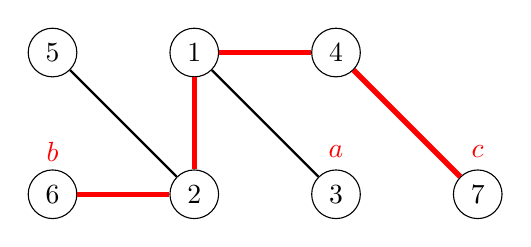
\begin{tikzpicture}[scale=0.9]
        \node[draw, circle] (1) at (0,3) {$1$};
        \node[draw, circle] (2) at (2,3) {$4$};
        \node[draw, circle] (3) at (0,1) {$2$};
        \node[draw, circle] (4) at (2,1) {$3$};
        \node[draw, circle] (5) at (4,1) {$7$};
        \node[draw, circle] (6) at (-2,3) {$5$};
        \node[draw, circle] (7) at (-2,1) {$6$};
        \path[draw,thick,-] (1) -- (2);
        \path[draw,thick,-] (1) -- (3);
        \path[draw,thick,-] (1) -- (4);
        \path[draw,thick,-] (2) -- (5);
        \path[draw,thick,-] (3) -- (6);
        \path[draw,thick,-] (3) -- (7);
        \node[color=red] at (2,1.6) {$a$};
        \node[color=red] at (-2,1.6) {$b$};
        \node[color=red] at (4,1.6) {$c$};

        \path[draw,thick,-,color=red,line width=2pt] (7) -- (3);
        \path[draw,thick,-,color=red,line width=2pt] (3) -- (1);
        \path[draw,thick,-,color=red,line width=2pt] (1) -- (2);
        \path[draw,thick,-,color=red,line width=2pt] (2) -- (5);
    \end{tikzpicture}
\end{center}

Este es un elegante método, pero, ¿por qué funciona?

Ayuda si dibujamos el árbol de tal manera que el camino que
corresponde al diámetro sea horizontal, y todos los otros nodos
se ``cuelguen'' de él:
\begin{center}
    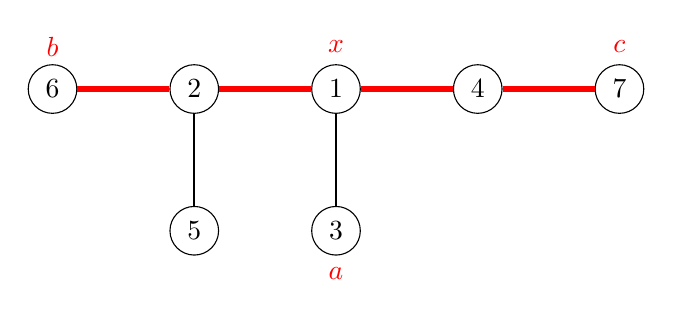
\begin{tikzpicture}[scale=0.9]
        \node[draw, circle] (1) at (2,1) {$1$};
        \node[draw, circle] (2) at (4,1) {$4$};
        \node[draw, circle] (3) at (0,1) {$2$};
        \node[draw, circle] (4) at (2,-1) {$3$};
        \node[draw, circle] (5) at (6,1) {$7$};
        \node[draw, circle] (6) at (0,-1) {$5$};
        \node[draw, circle] (7) at (-2,1) {$6$};
        \path[draw,thick,-] (1) -- (2);
        \path[draw,thick,-] (1) -- (3);
        \path[draw,thick,-] (1) -- (4);
        \path[draw,thick,-] (2) -- (5);
        \path[draw,thick,-] (3) -- (6);
        \path[draw,thick,-] (3) -- (7);
        \node[color=red] at (2,-1.6) {$a$};
        \node[color=red] at (-2,1.6) {$b$};
        \node[color=red] at (6,1.6) {$c$};
        \node[color=red] at (2,1.6) {$x$};

        \path[draw,thick,-,color=red,line width=2pt] (7) -- (3);
        \path[draw,thick,-,color=red,line width=2pt] (3) -- (1);
        \path[draw,thick,-,color=red,line width=2pt] (1) -- (2);
        \path[draw,thick,-,color=red,line width=2pt] (2) -- (5);
    \end{tikzpicture}
\end{center}

Un nodo $x$ indica el lugar donde el camino desde el nodo $a$
se une con el camino que corresponde al diámetro. El nodo más
lejano de $a$ es el nodo $b$, $c$, o cualquier otro que esté
por lo menos igual de lejos $x$. Por lo tanto,
este nodo siempre es una opción válida para un extremo del
camino que corresponde al diámetro.

\section{Todos los caminos máximos}

Nuestro siguiente problema es calcular, para cada nodo en el árbol,
la longitud máxima de un camino que comienza en el nodo. Podemos verlo
como una generalización del problema del diámetro del árbol,
porque el más largo de estos caminos es igual al diámetro.
Este problema puede resolverse en $O(n)$.

Por ejemplo, considera el siguiente árbol:
\begin{center}
    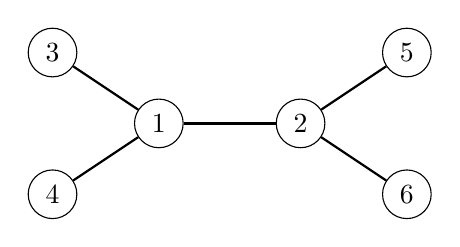
\begin{tikzpicture}[scale=0.9]
        \node[draw, circle] (1) at (0,0) {$1$};
        \node[draw, circle] (2) at (-1.5,-1) {$4$};
        \node[draw, circle] (3) at (2,0) {$2$};
        \node[draw, circle] (4) at (-1.5,1) {$3$};
        \node[draw, circle] (6) at (3.5,-1) {$6$};
        \node[draw, circle] (7) at (3.5,1) {$5$};
        \path[draw,thick,-] (1) -- (2);
        \path[draw,thick,-] (1) -- (3);
        \path[draw,thick,-] (1) -- (4);
        \path[draw,thick,-] (3) -- (6);
        \path[draw,thick,-] (3) -- (7);
    \end{tikzpicture}
\end{center}

Digamos que $\texttt{long\_max}(x)$ denota la longitud máxima
de un camino que comienza en el nodo $x$. Por ejemplo, en el
árbol de arriba, $\texttt{long\_max}(4)=3$, porque hay un camino
$4 \rightarrow 1 \rightarrow 2 \rightarrow 6$. Aquí vemos una
tabla completa de los valores:
\begin{center}
    \begin{tabular}{l|lllllll}
        nodo $x$                & 1 & 2 & 3 & 4 & 5 & 6 \\
        $\texttt{long\_max}(x)$ & 2 & 2 & 3 & 3 & 3 & 3 \\
    \end{tabular}
\end{center}

También en este problema, un buen punto de partida para resolverlo
es asignarle una raíz al árbol arbitrariamente:
\begin{center}
    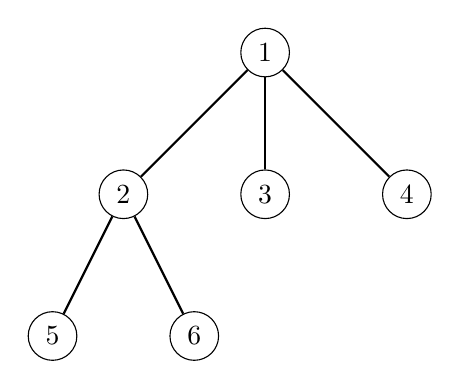
\begin{tikzpicture}[scale=0.9]
        \node[draw, circle] (1) at (0,3) {$1$};
        \node[draw, circle] (2) at (2,1) {$4$};
        \node[draw, circle] (3) at (-2,1) {$2$};
        \node[draw, circle] (4) at (0,1) {$3$};
        \node[draw, circle] (6) at (-3,-1) {$5$};
        \node[draw, circle] (7) at (-1,-1) {$6$};
        \path[draw,thick,-] (1) -- (2);
        \path[draw,thick,-] (1) -- (3);
        \path[draw,thick,-] (1) -- (4);
        \path[draw,thick,-] (3) -- (6);
        \path[draw,thick,-] (3) -- (7);
    \end{tikzpicture}
\end{center}

La primera parte del problema es calcular para cada nodo $x$ la
longitud máxima de un camino que pasa por un hijo de $x$.
Por ejemplo, el camino más largo del nodo 1 pasa por su hijo 2:
\begin{center}
    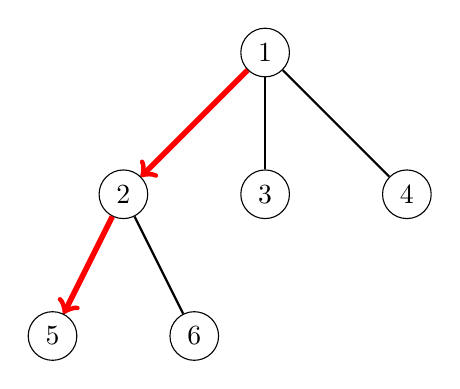
\begin{tikzpicture}[scale=0.9]
        \node[draw, circle] (1) at (0,3) {$1$};
        \node[draw, circle] (2) at (2,1) {$4$};
        \node[draw, circle] (3) at (-2,1) {$2$};
        \node[draw, circle] (4) at (0,1) {$3$};
        \node[draw, circle] (6) at (-3,-1) {$5$};
        \node[draw, circle] (7) at (-1,-1) {$6$};
        \path[draw,thick,-] (1) -- (2);
        \path[draw,thick,-] (1) -- (3);
        \path[draw,thick,-] (1) -- (4);
        \path[draw,thick,-] (3) -- (6);
        \path[draw,thick,-] (3) -- (7);

        \path[draw,thick,->,color=red,line width=2pt] (1) -- (3);
        \path[draw,thick,->,color=red,line width=2pt] (3) -- (6);
    \end{tikzpicture}
\end{center}
Esta parte es fácil de resolver en $O(n)$, porque podemos utilizar
la programación dinámica como hemos hecho previamente.

Entonces, la segunda parte del problema es calcular para cada
nodo $x$ la longitud máxima de un camino que pase por su padre $p$.
Por ejemplo, el camino más largo desde el nodo 3 pasa por su padre 1:
\begin{center}
    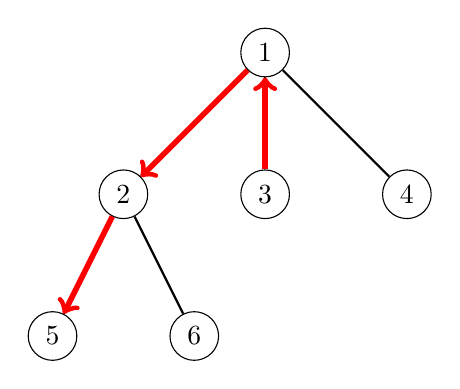
\begin{tikzpicture}[scale=0.9]
        \node[draw, circle] (1) at (0,3) {$1$};
        \node[draw, circle] (2) at (2,1) {$4$};
        \node[draw, circle] (3) at (-2,1) {$2$};
        \node[draw, circle] (4) at (0,1) {$3$};
        \node[draw, circle] (6) at (-3,-1) {$5$};
        \node[draw, circle] (7) at (-1,-1) {$6$};
        \path[draw,thick,-] (1) -- (2);
        \path[draw,thick,-] (1) -- (3);
        \path[draw,thick,-] (1) -- (4);
        \path[draw,thick,-] (3) -- (6);
        \path[draw,thick,-] (3) -- (7);

        \path[draw,thick,->,color=red,line width=2pt] (4) -- (1);
        \path[draw,thick,->,color=red,line width=2pt] (1) -- (3);
        \path[draw,thick,->,color=red,line width=2pt] (3) -- (6);
    \end{tikzpicture}
\end{center}

A primera vista, parece que deberíamos elegir el camino más
largo desde $p$. Sin embargo, esto \emph{no} siempre funciona,
porque el camino más largo de $p$ puede pasar por $x$. Aquí
vemos un ejemplo de esta situación:
\begin{center}
    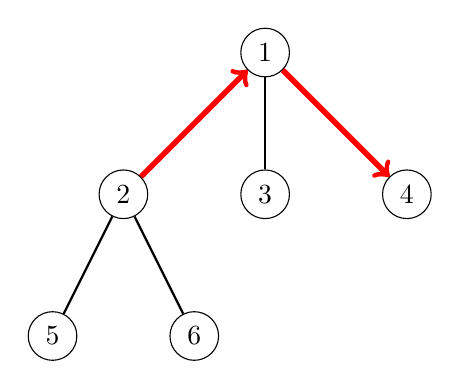
\begin{tikzpicture}[scale=0.9]
        \node[draw, circle] (1) at (0,3) {$1$};
        \node[draw, circle] (2) at (2,1) {$4$};
        \node[draw, circle] (3) at (-2,1) {$2$};
        \node[draw, circle] (4) at (0,1) {$3$};
        \node[draw, circle] (6) at (-3,-1) {$5$};
        \node[draw, circle] (7) at (-1,-1) {$6$};
        \path[draw,thick,-] (1) -- (2);
        \path[draw,thick,-] (1) -- (3);
        \path[draw,thick,-] (1) -- (4);
        \path[draw,thick,-] (3) -- (6);
        \path[draw,thick,-] (3) -- (7);

        \path[draw,thick,->,color=red,line width=2pt] (3) -- (1);
        \path[draw,thick,->,color=red,line width=2pt] (1) -- (2);
    \end{tikzpicture}
\end{center}

De todas formas, podemos resolver la segunda parte en $O(n)$
si almacenamos \emph{dos} longitudes máximas por cada nodo $x$:
\begin{itemize}
    \item $\texttt{long\_max}_1(x)$:
          la longitud máxima de un camino desde $x$
    \item $\texttt{long\_max}_2(x)$:
          la longitud máxima de un camino desde $x$
          en otra dirección que la del primer camino
\end{itemize}
Por ejemplo, en el grafo de arriba,
$\texttt{long\_max}_1(1)=2$
utilizando el camino $1 \rightarrow 2 \rightarrow 5$,
y $\texttt{long\_max}_2(1)=1$
utilizando el camino $1 \rightarrow 3$.

Finalmente, si el camino que corresponde a $\texttt{long\_max}_1(p)$
pasa por $x$, concluimos que la longitud máxima es
$\texttt{long\_max}_2(p)+1$, y de lo contrario la longitud máxima es
$\texttt{long\_max}_1(p)+1$.

\section{Árboles binarios}

\index{árbol binario}

\begin{samepage}

    Un \key{árbol binario} es un árbol con raíz donde cada nodo
    tiene un subárbol izquierdo y derecho. Es posible que algún subárbol
    esté vacío. Por ende, cada nodo en un árbol binario tiene cero, uno,
    o dos hijos.

    Por ejemplo, el siguiente árbol es un árbol binario:
    \begin{center}
        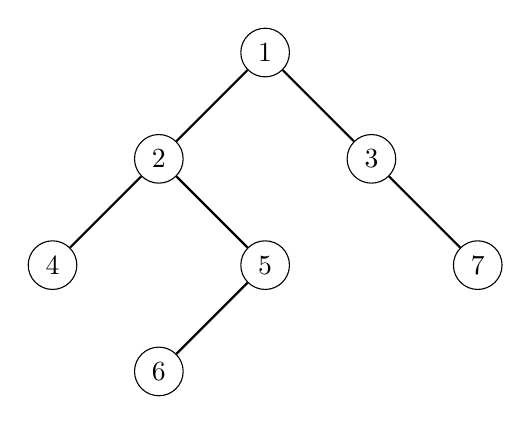
\begin{tikzpicture}[scale=0.9]
            \node[draw, circle] (1) at (0,0) {$1$};
            \node[draw, circle] (2) at (-1.5,-1.5) {$2$};
            \node[draw, circle] (3) at (1.5,-1.5) {$3$};
            \node[draw, circle] (4) at (-3,-3) {$4$};
            \node[draw, circle] (5) at (0,-3) {$5$};
            \node[draw, circle] (6) at (-1.5,-4.5) {$6$};
            \node[draw, circle] (7) at (3,-3) {$7$};

            \path[draw,thick,-] (1) -- (2);
            \path[draw,thick,-] (1) -- (3);
            \path[draw,thick,-] (2) -- (4);
            \path[draw,thick,-] (2) -- (5);
            \path[draw,thick,-] (5) -- (6);
            \path[draw,thick,-] (3) -- (7);
        \end{tikzpicture}
    \end{center}
\end{samepage}

\index{preorden}
\index{inorden}
\index{postorden}

Los nodos de un árbol binario tienen tres ordenamientos naturales
que corresponden a las diferentes maneras de recorrer el árbol
recursivamente:

\begin{itemize}
    \item \key{preorden}: primero procesamos la raíz, luego recorremos el
          subárbol izquierdo, luego el subárbol derecho
    \item \key{inorden}: primero recorremos el subárbol izquierdo,
          luego procesamos la raíz, luego recorremos el subárbol derecho
    \item \key{postorden}: primero recorremos el subárbol izquierdo,
          luego el subárbol derecho, luego procesamos la raíz
\end{itemize}

Para el árbol de arriba, los nodos en preorden son $[1,2,4,5,6,3,7]$,
en inorden son $[4,2,6,5,1,3,7]$, y en postorden son $[4,6,5,2,7,3,1]$.

Si sabemos el preorden e inorden de un árbol, podemos reconstruir la
estructura exacta del mismo. Por ejemplo, el árbol de arriba es el único
árbol posible con preorden $[1,2,4,5,6,3,7]$ e inorden $[4,2,6,5,1,3,7]$.
Similarmente, el postorden e inorden también determinan la estructura
de un árbol.

Sin embargo, la situación es diferente si solamente sabemos el preorden
y postorden de un árbol. En este caso, pueden haber múltiples árboles
posibles. Por ejemplo, en los dos siguientes árboles
\begin{center}
    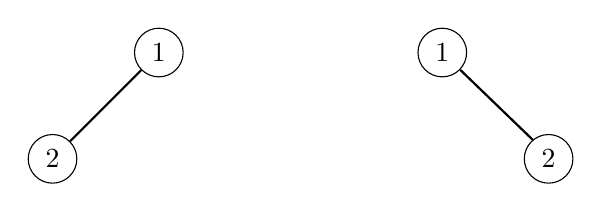
\begin{tikzpicture}[scale=0.9]
        \node[draw, circle] (1) at (0,0) {$1$};
        \node[draw, circle] (2) at (-1.5,-1.5) {$2$};
        \path[draw,thick,-] (1) -- (2);

        \node[draw, circle] (1b) at (0+4,0) {$1$};
        \node[draw, circle] (2b) at (1.5+4,-1.5) {$2$};
        \path[draw,thick,-] (1b) -- (2b);
    \end{tikzpicture}
\end{center}
el preorden es $[1,2]$ y el postorden es $[2,1]$,
pero sus estructuras son diferentes.
